
%(BEGIN_QUESTION)
% Copyright 2006, Tony R. Kuphaldt, released under the Creative Commons Attribution License (v 1.0)
% This means you may do almost anything with this work of mine, so long as you give me proper credit

Tre ulike utforminger av globeventiler vises her: {\it stem-guided}, {\it port-guided} og {\it cage-guided}:

$$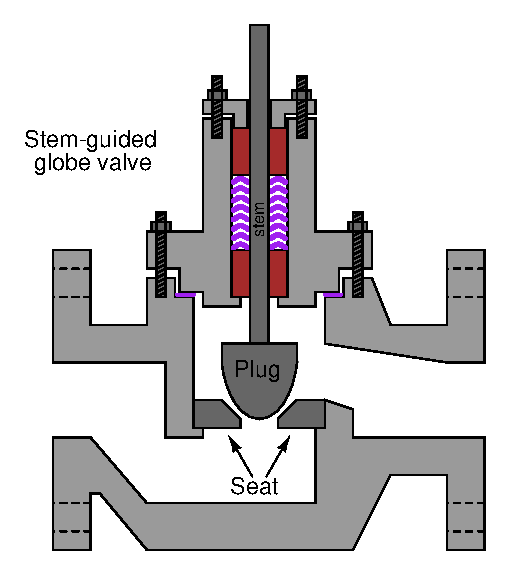
\includegraphics[width=5cm]{i00775x01.eps}$$

$$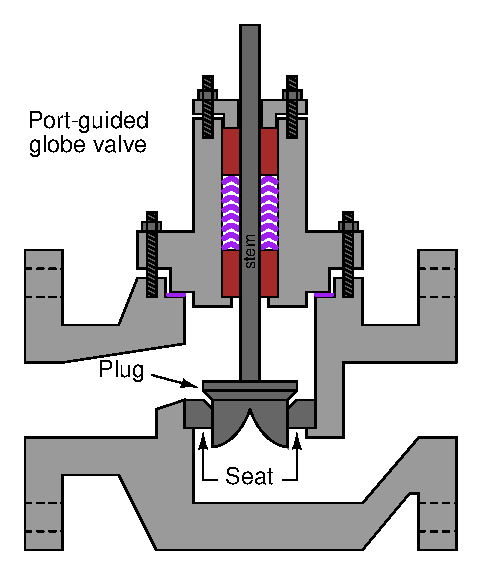
\includegraphics[width=5cm]{i00775x02.eps}$$

$$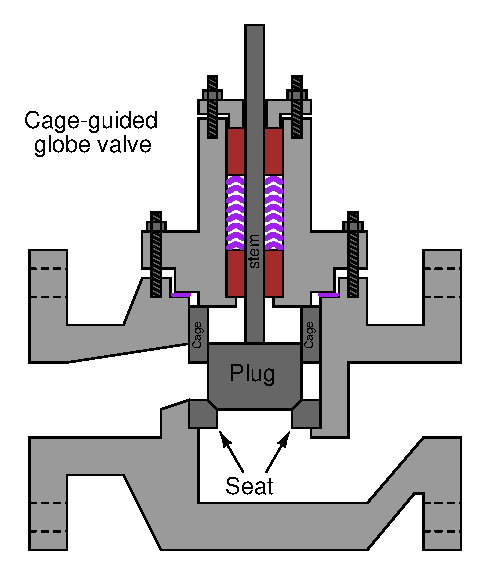
\includegraphics[width=5cm]{i00775x03.eps}$$

Beskriv forskjellene mellom disse tre globeventildesignene, og angi hvilken som er mest utbredt i industrien i dag.

\underbar{file i00775}
%(END_QUESTION)





%(BEGIN_ANSWER)

Cage-guided-ventildesignet er det mest utbredte i dag.

\vskip 10pt

I en cage-ventil strupes strømningen ikke av åpningen mellom en profilert plugg og setet, men av åpningene i buret som avdekkes av den stempelformede pluggen. Setet har i praksis kun én oppgave: tett avstenging ved 0\% åpen (helt lukket).

Siden dette er tilfellet, utsettes setet i en cage-ventil for mindre slitasje enn i globeventiler med profilert plugg eller «v-ported» plugg, noe som forlenger levetiden. Ventilens åpningskarakteristikk (hurtigåpnende, lineær, lik-prosent) kan lett endres ved å bytte bare buret. I en vanlig globeventil må pluggen byttes til annen profil. Fordi bur vanligvis er enklere å bytte enn plugger, gir dette bedre fleksibilitet.

%(END_ANSWER)





%(BEGIN_NOTES)


%INDEX% Sluttkontrollelementer, ventil: guiding av globeventiler (spindel, port og bur)

%(END_NOTES)


